\section{Technology}
The experiment in this project report utilized a web server and a search engine as the backend.

NodeJS\footnote{\url{https://nodejs.org}} v7 was chosen as the webserver.
NodeJS was chosen because the author has knowledge of the technology,
and it contains a rich package manager called NPM.
By utilizing open source libraries through NPM, more time could be spent implementing the algoritms for query expansion.
Inside NodeJS lies the V8\footnote{\url{https://developers.google.com/v8/}} JavaScript engine.

Elasticsearch\footnote{\url{https://www.elastic.co/products/elasticsearch}} v5 were utilized as the search engine.
At the time of writing Elasticsearch is a popular open source search engines, which has proven the ability to scale up to petabytes of data \cite{elasticsearch-scale}.
Elasticsearch is open source and built on top of Lucene\footnote{\url{https://lucene.apache.org/}}.
Lucene is the search engine itself,
and Elasticsearch provides functionality for distribution and a REST API interface.

\subsection{Lucene}

\subsection{Elasticsearch}
Elasticsearch Machine Learning in Beta as of may https://www.elastic.co/products/x-pack.
elasticsearch vs solr

[??] descibe cluster
[??] explain different node types

\subsubsection{Sharding}
The stored in Elasticsearch may grow to become larger then the hardware on a single machine can handle,
both in size and in number of requests.
To handle the problem elasticsearch splits each index into multiple segments called shards.
Each of this shards may be distributed across multiple nodes.
This leads to higher performance when indexing new documents and when searching the documents.
The shards may also be duplicated to support higher query volumes and availability.

However, when the cluster consists of multiple nodes a query strategy is required.
Figure \ref{fig:elasticsearch-sharding} illustrates how an index may be distributed across three nodes.
The figure shows a simplified view on how a query are distributed across three nodes.
First the query arrives a handler node [??check type].
The handler node parses the query and determines which nodes holds shards for the given index.
Each shard determines locally which documents are most relevant from the query.
Metada from all the shards are then sent back to the handler node.
On the handler node alle the retrieved metadata are used to calculate the global result.
After the global result have been calculated,
all the shards are then queried for the documents from the global result.
After the documents are retrieved the result are returned back to the client.

\begin{figure}[h!]
  \centering 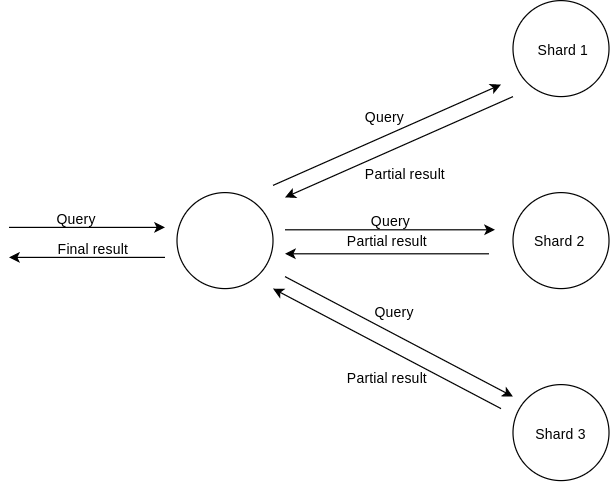
\includegraphics[width=0.9\linewidth]{img/elasticsearch-sharding.png}
  \caption{Elasticsearch distributing query agains all the shards}
  \label{fig:elasticsearch-sharding}
\end{figure}

Because of Elasticsearch's distributed nature
https://www.elastic.co/guide/en/elasticsearch/reference/current/search-aggregations-bucket-terms-aggregation.html
